\documentclass[11pt]{article}
\usepackage[utf8]{inputenc}
\usepackage[T1]{fontenc}
\usepackage[margin=1in]{geometry}
\usepackage{amsmath,amssymb,amsthm}
\usepackage{booktabs}
\usepackage{array}
\usepackage{url}
\usepackage{microtype}
\usepackage{graphicx}
\usepackage{caption}
\usepackage{fancyvrb}
\usepackage[hidelinks]{hyperref}
\makeatletter\g@addto@macro{\UrlBreaks}{\do\_\do\.}\makeatother
\DeclareUrlCommand\lean{\urlstyle{tt}}
\emergencystretch=3em
\DeclareUnicodeCharacter{00AC}{\ensuremath{\neg}}
\DeclareUnicodeCharacter{00B7}{\ensuremath{\cdot}}
\DeclareUnicodeCharacter{00B9}{\ensuremath{^{1}}}
\DeclareUnicodeCharacter{03B9}{\ensuremath{\iota}}
\DeclareUnicodeCharacter{03BA}{\ensuremath{\kappa}}
\DeclareUnicodeCharacter{03C1}{\ensuremath{\rho}}
\DeclareUnicodeCharacter{2016}{\ensuremath{\Vert}}
\DeclareUnicodeCharacter{2022}{\ensuremath{\bullet}}
\DeclareUnicodeCharacter{207B}{\ensuremath{^{-}}}
\DeclareUnicodeCharacter{2115}{\ensuremath{\mathbb{N}}}
\DeclareUnicodeCharacter{211D}{\ensuremath{\mathbb{R}}}
\DeclareUnicodeCharacter{2190}{\ensuremath{\leftarrow}}
\DeclareUnicodeCharacter{2192}{\ensuremath{\to}}
\DeclareUnicodeCharacter{2200}{\ensuremath{\forall}}
\DeclareUnicodeCharacter{2208}{\ensuremath{\in}}
\DeclareUnicodeCharacter{2211}{\ensuremath{\Sigma}}
\DeclareUnicodeCharacter{221E}{\ensuremath{\infty}}
\DeclareUnicodeCharacter{2227}{\ensuremath{\wedge}}
\DeclareUnicodeCharacter{2260}{\ensuremath{\ne}}
\DeclareUnicodeCharacter{2264}{\ensuremath{\le}}
\DeclareUnicodeCharacter{2265}{\ensuremath{\ge}}
\DeclareUnicodeCharacter{22A4}{\ensuremath{\top}}
\DeclareUnicodeCharacter{1D4DD}{\ensuremath{\mathcal{N}}}

\newcommand{\ROne}{40}
\newcommand{\ETriOne}{1.6253213396063}
\newcommand{\ESqOne}{1.6348554953172}
\newcommand{\SfTriOne}{1.6076092171853}
\newcommand{\SfSqOne}{1.6171455730029}
\newcommand{\DTriOne}{1.7712\times10^{-2}}
\newcommand{\DSqOne}{1.7710\times10^{-2}}
\newcommand{\TailOne}{5.6\times10^{-17}}
\newcommand{\GapExOne}{9.534156\times10^{-3}}
\newcommand{\GapSfOne}{9.536356\times10^{-3}}
\newcommand{\GapChOne}{-2.20\times10^{-6}}
\newcommand{\TwiceTriOne}{3.2506426792}
\newcommand{\BoxDiffOne}{2.2\times10^{-16}}
\newcommand{\SelfImgOne}{5.16\times10^{-9}}
\newcommand{\SadNegOne}{64}
\newcommand{\SadAfterOne}{2.856510\times10^{-3}}
\newcommand{\RTwo}{20}
\newcommand{\ETriTwo}{0.3935428489324}
\newcommand{\ESqTwo}{0.4009742487651}
\newcommand{\SfTriTwo}{0.3935333668255}
\newcommand{\SfSqTwo}{0.4009647698931}
\newcommand{\DTriTwo}{9.4821\times10^{-6}}
\newcommand{\DSqTwo}{9.4789\times10^{-6}}
\newcommand{\TailTwo}{1.2\times10^{-16}}
\newcommand{\GapExTwo}{7.431400\times10^{-3}}
\newcommand{\GapSfTwo}{7.431403\times10^{-3}}
\newcommand{\GapChTwo}{-3.24\times10^{-9}}
\newcommand{\TwiceTriTwo}{0.7870856979}
\newcommand{\BoxDiffTwo}{5.6\times10^{-17}}
\newcommand{\SelfImgTwo}{2.36\times10^{-16}}
\newcommand{\SadNegTwo}{72}
\newcommand{\SadAfterTwo}{2.224729\times10^{-3}}
\newcommand{\MpMaxRust}{1.7\times10^{-16}}
\newcommand{\MpMaxEwald}{5.2\times10^{-29}}
\newcommand{\MpMaxTextbook}{1.5\times10^{-14}}
\newcommand{\MpDps}{40}
\newcommand{\NRelax}{24}
\newcommand{\NRelaxOne}{11}
\newcommand{\NRelaxTwo}{13}
\newcommand{\NBelow}{0}
\newcommand{\NZeroGap}{1}
\newcommand{\ZeroGapStage}{$\kappa=1$ \texttt{uniform\_00} anneal quench}
\newcommand{\TriBoxDiffOne}{-2.2\times10^{-16}}
\newcommand{\OcMtime}{2026-10-10 20:04}
\newcommand{\NNegModes}{0}
\newcommand{\NSfRepro}{24}
\newcommand{\NConv}{24}
\newcommand{\MaxGapChOne}{5.3\times10^{-7}}
\newcommand{\MaxGapChTwo}{3.0\times10^{-10}}
\newcommand{\MinGapOne}{4.584\times10^{-4}}
\newcommand{\OcRev}{6a1dfef12aec878b4cda99edd54b16a6a254e135}
\newcommand{\OcSha}{9e4249ba20cf4cdc46f69e7fe6deb19be286dd19c9f1cf85d350816d2b1e748b}
\newcommand{\OcBytes}{142986687}
\newcommand{\OcLicense}{CC-BY-4.0}
\newcommand{\SigMin}{9.76\times10^{-3}}
\newcommand{\MixQuarter}{-0.2585}
\newcommand{\RcYk}{0}
\newcommand{\SecYk}{1074.1}
\newcommand{\RcMix}{0}
\newcommand{\SecMix}{22.1}
\newcommand{\RcYkCtl}{0}
\newcommand{\SecYkCtl}{18.1}
\newcommand{\RcMixCtl}{0}
\newcommand{\SecMixCtl}{18.6}
\newcommand{\RcVer}{0}
\newcommand{\SecVer}{21.4}
\newcommand{\LedgerExit}{1}
\newcommand{\LedgerClaims}{25}
\newcommand{\LedgerBlocks}{0}
\newcommand{\LedgerFlags}{11}
\newcommand{\LedgerNA}{11}
\newcommand{\LedgerNL}{5}
\newcommand{\LedgerNC}{3}
\newcommand{\LedgerNX}{6}

\newtheorem{theorem}{Theorem}
\newtheorem{lemma}[theorem]{Lemma}
\newtheorem{definition}[theorem]{Definition}
\theoremstyle{remark}
\newtheorem{step}{Step}
\newcommand{\R}{\mathbb{R}}
\newcommand{\tier}[1]{\textbf{[#1]}}

\title{The triangular lattice minimises the planar Yukawa energy at every density\\ and for every finite mixture of screening lengths:
kernel-checked corollaries of planar universal optimality,\\ a human proof, and an exact-potential CVODE consistency study}
\author{Xavier Callens (SocrateAI Lab)\thanks{AI-assistance disclosure: this preprint, its Lean files, its code and
its ledger were produced by AI agents (Claude, Anthropic) under the author's direction. The author is responsible for
the content. No human expert has reviewed it.}}
\date{Preprint v1, 2026-10-25}
\hypersetup{pdftitle={Triangular lattice minimises the planar Yukawa energy}, pdfauthor={Xavier Callens}}

\begin{document}
\maketitle
\begin{center}\small doi:10.5281/zenodo.23646105 \quad (not peer reviewed)\end{center}


\begin{abstract}
The openai/math release contains a Lean~4 proof (AI-generated, Comparator-accepted, not peer reviewed) that the
triangular lattice minimises the lower $g$-energy among all locally finite planar configurations of density one, for
every smooth completely monotone $g$ of squared distance~\cite{oai}. We apply it to the \emph{planar Yukawa}
interaction $V(r)=e^{-\kappa r}/r$, the three-dimensional screened Coulomb potential between particles confined to a
plane, as in two-dimensional dusty-plasma and colloidal crystals. It is not the Green function $K_0(\kappa r)$ of the
2D Debye--H\"uckel equation, which we do not treat. At \tier{A} (kernel-checked, axioms within
\texttt{propext}, \texttt{Classical.choice}, \texttt{Quot.sound}, planted controls caught), conditional on upstream's
theorem and on the fidelity of its definitions, we prove:
(i) $V$ is admissible for every $\kappa>0$, so the triangular lattice minimises its energy at density one, and that
minimum is finite;
(ii) the same holds at every density $\rho>0$ for the rescaled lattice;
(iii) the same holds for every finite mixture $\sum_i w_i e^{-\kappa_i r}/r$ with $w_i\ge 0$, $\kappa_i>0$; and
(iv) the admissibility lemma needs the sign condition: $g_1-2g_2$ is not admissible, so the theorem does not apply
to it (this does not show that optimality fails for it).
The mathematics is classical; only the kernel-checked corollaries are new. We give a step-by-step human proof
\tier{C} beside each Lean statement. At \tier{X} (floating point, never evidence for a claim) we correct a published
truncation erratum: with the exact, untruncated potential and a rigorous tail bound, CVODE re-relaxations of
\NRelax{} published stages find none below the exact triangular energy beyond f64 resolution. The Elenchus ledger gate reports
\LedgerBlocks{} blocking findings and \LedgerFlags{} flags (exit~\LedgerExit). Each flag is a Tier~A row whose
statement adequacy no human has audited.
\end{abstract}

\section{Claims and tiers}\label{sec:claims}

We use the tiers of the SocrateAI-Scientific-Elenchus method~\cite{elenchus}. \tier{A}: a Lean theorem compiled under
the pinned toolchain whose \verb|#print axioms| footprint is within the allowlist, with planted \texttt{sorry} and
planted-axiom controls caught. \tier{L}: a verified literature source, quoted with line numbers. Our L rows cite a
definition, a convention, a remark and a footnote. Elenchus's \texttt{citation\_check.py} accepts only theorems,
lemmas, propositions and corollaries, so it would refuse them on kind alone; the quotations were checked instead
against the alphaXiv full text of arXiv:1902.05438 (and, for YK-L-0003, the pinned upstream source), by the producer
and again by an independent auditor. \tier{C}: an
argument or proof that no machine checked. \tier{X}: a floating-point computation. It may steer the work and may
never support a claim. Tier~A certifies a Lean statement about Lean definitions, not its physical reading. Every
Tier~A optimality statement here rests on upstream's \lean{universal_energy_minimum}.

\begin{table}[!ht]\centering\small
\begin{tabular}{>{\raggedright\arraybackslash}p{2.2cm}p{0.7cm}p{11.7cm}}
\toprule
Ledger id & Tier & Claim (abbreviated; full statements in \texttt{ledger/ledger.json}) \\
\midrule
YK-A-0001--3 & A & upstream \lean{universal_energy_minimum}; Riesz admissibility and finiteness for $s>2$; every-density form (D2)~\cite{d12}\\
YK-A-0004 & A & products and restriction: \lean{admissible_mul}, \lean{admissible_congr}; $e^{-\kappa\sqrt t}$ admissible\\
YK-A-0005--6 & A & planar Yukawa admissible and triangular-optimal at density one; lattice energy finite\\
YK-A-0007, 11 & A & negative controls: $e^{-\kappa\sqrt t}\cos t$ and $g_1-2g_2$ are not admissible\\
YK-A-0008 & A & closure under sums, nonnegative multiples, finite nonnegative combinations\\
YK-A-0009 & A & every density $\rho>0$, finite minimum; scaling identity (pointwise)\\
YK-A-0010 & A & finite mixtures of screening lengths: admissible, optimal at density one and every density, finite\\
YK-L-0001--5 & L & CKMRV Def.~1.3, lattice-energy convention, composition footnote, vacancy remark~\cite{ckmrv}; upstream scope remark~\cite{oai}\\
YK-C-0001 & C & the human demonstration of Section~\ref{sec:human}\\
YK-C-0002 & C & the physics reading (Section~\ref{sec:physics}), including the factor-2 convention\\
YK-C-0003 & C & no dusty-plasma or colloid particle dataset on the Hugging Face Hub (absence by search)\\
YK-X-0001--6 & X & exact-potential energies, controls, relaxations, OC20 provenance, sampled sign checks\\
\bottomrule
\end{tabular}
\caption{The claim ledger: \LedgerClaims{} rows (\LedgerNA{} A, \LedgerNL{} L, \LedgerNC{} C, \LedgerNX{} X). Every row
points to a content-addressed evidence blob. The gate checks that no row is filed above anything it rests on,
transitively.}\label{tab:ledger}
\end{table}

\section{Setting: upstream's definitions}\label{sec:setting}

A potential is a function $g:\R\to\R$ of the \emph{squared} distance $t=r^2$. Upstream's definitions, verbatim from
the pinned openai/math source~\cite{oai}, are:
\begin{Verbatim}[fontsize=\scriptsize,frame=single,framesep=1.5mm]
def AdmissiblePotential (g : ℝ → ℝ) : Prop :=
  ContDiffOn ℝ (⊤ : ℕ∞) g (Set.Ioi 0) ∧
  (∀ t : ℝ, 0 < t → 0 ≤ g t) ∧
  ∀ (r : ℕ) (t : ℝ), 0 < t → 0 ≤ (-1 : ℝ) ^ r * iteratedDeriv r g t

def diskEnergy (g : ℝ → ℝ) (C : Set Plane) (R : ℝ) : ℝ≥0∞ :=
  (diskCount C R : ℝ≥0∞)⁻¹ *
    ∑ x ∈ diskPoints C R, ∑ y ∈ (diskPoints C R).erase x,
      ENNReal.ofReal (g (‖x - y‖ ^ 2))

def energy (g : ℝ → ℝ) (C : Set Plane) : ℝ≥0∞ :=
  Filter.liminf (diskEnergy g C) atTop

def latticeEnergy (g : ℝ → ℝ) : ℝ≥0∞ :=
  ∑' a : {x : Plane // x ∈ A ∧ x ≠ 0}, ENNReal.ofReal (g (‖a.val‖ ^ 2))

theorem universal_energy_minimum (g : ℝ → ℝ) (C : Set Plane)
    (hg : AdmissiblePotential g) (_hC : LocallyFinite C) (hd : DensityOne C) :
    latticeEnergy g ≤ energy g C ∧ latticeEnergy g = energy g A := by
\end{Verbatim}

\noindent So $g$ is \emph{admissible} if it is $C^\infty$ on $(0,\infty)$, nonnegative there, and
$(-1)^r g^{(r)}(t)\ge 0$ for every $r$ and $t>0$; that is, completely monotone on $(0,\infty)$. The energy of a
configuration $C$ is the $\liminf$ over $R\to\infty$ of the disk-averaged sum over \emph{ordered} pairs, and
\lean{latticeEnergy} sums over the nonzero vectors of the density-one triangular lattice $A$ (nearest-neighbour
spacing $a=\sqrt{2/\sqrt3}$). Neither carries a factor $\tfrac12$, the same convention as CKMRV \tier{L}~\cite{ckmrv}.
The every-density form~\cite{d12} uses:
\begin{Verbatim}[fontsize=\scriptsize,frame=single,framesep=1.5mm]
def DensityRho (ρ : ℝ) (C : Set Plane) : Prop :=
  Tendsto (fun R : ℝ => (diskCount C R : ℝ) / (Real.pi * R ^ 2)) atTop (𝓝 ρ)

theorem universal_any_density (h : ℝ → ℝ) (hh : AdmissiblePotential h) {ρ : ℝ} (hρ : 0 < ρ) (C : Set Plane)
    (hC : LocallyFinite C) (hd : DensityRho ρ C) :
    latticeEnergy (fun t => h (ρ⁻¹ * t)) ≤ energy h C := by
\end{Verbatim}

\noindent Our definitions (\texttt{formal\_cert/Autoresearch/Yukawa.lean}):
\begin{Verbatim}[fontsize=\scriptsize,frame=single,framesep=1.5mm]
noncomputable def phi (κ : ℝ) : ℝ → ℝ := fun t => Real.exp (-κ * Real.sqrt t)

noncomputable def g (κ : ℝ) : ℝ → ℝ := fun t => Real.exp (-κ * Real.sqrt t) / Real.sqrt t

noncomputable def c (κ : ℝ) : ℝ → ℝ := fun t => Real.exp (-κ * Real.sqrt t) * Real.cos t
\end{Verbatim}


\section{Human mathematical demonstration}\label{sec:human}

This section is a complete proof written for a strong undergraduate. The prose is \tier{C}: no machine checked it.
After each step we give the Lean statement that the kernel did check \tier{A}. Throughout, $\kappa>0$, $t>0$, and
$f^{(n)}$ is the $n$-th derivative. We say $f$ has the \emph{sign pattern up to order $n$} at $t$ if
$(-1)^i f^{(i)}(t)\ge0$ for $i=0,\dots,n$.

\begin{step}[$t^{-1/2}$ is admissible]
For $s>0$ let $p(t)=t^{-s/2}$. By induction,
$p^{(n)}(t)=(-1)^n \tfrac{s}{2}\big(\tfrac{s}{2}+1\big)\cdots\big(\tfrac{s}{2}+n-1\big)\,t^{-s/2-n}$: differentiating
$t^{-\alpha}$ gives $-\alpha t^{-\alpha-1}$, and each step adds one factor $-(\tfrac s2+k)<0$. The product of
positive numbers times $t^{-s/2-n}>0$ is positive, so $(-1)^np^{(n)}(t)>0$. The function is smooth on $(0,\infty)$ as
a real power of a positive variable. With $s=1$, $t^{-1/2}$ is admissible.
\emph{Lean (prior work~\cite{d12}):} \lean{TriangularRiesz.riesz_admissible}, for \lean{riesz s t = t^(-(s/2))}.
\end{step}

\begin{step}[Leibniz sign lemma]
If $f$ and $h$ are $n$ times differentiable at $t$ and both have the sign pattern up to order $n$ at $t$, then
$(-1)^n(fh)^{(n)}(t)\ge0$. \emph{Proof.} Leibniz's rule gives
$(fh)^{(n)}=\sum_{i=0}^n\binom ni f^{(i)}h^{(n-i)}$. Write $(-1)^n=(-1)^i(-1)^{n-i}$. Then
$(-1)^n(fh)^{(n)}=\sum_i\binom ni\,\big[(-1)^if^{(i)}\big]\big[(-1)^{n-i}h^{(n-i)}\big]$, a sum of products of
nonnegative numbers. Applying this at every order shows that \emph{the product of two admissible functions is
admissible}; smoothness and nonnegativity of a product are immediate. Lean:
\end{step}
\begin{Verbatim}[fontsize=\scriptsize,frame=single,framesep=1.5mm]
lemma mul_sign {f h : ℝ → ℝ} {t : ℝ} (r : ℕ) (hf : ContDiffAt ℝ r f t) (hh : ContDiffAt ℝ r h t)
    (Hf : ∀ i ≤ r, 0 ≤ (-1 : ℝ) ^ i * iteratedDeriv i f t)
    (Hh : ∀ i ≤ r, 0 ≤ (-1 : ℝ) ^ i * iteratedDeriv i h t) :
    0 ≤ (-1 : ℝ) ^ r * iteratedDeriv r (f * h) t := by
  rw [iteratedDeriv_mul hf hh, Finset.mul_sum]
  refine Finset.sum_nonneg fun i hi => ?_
  have hir : i ≤ r := Nat.lt_succ_iff.mp (Finset.mem_range.mp hi)
  have hpow : (-1 : ℝ) ^ r = (-1) ^ i * (-1) ^ (r - i) := by
    rw [← pow_add, Nat.add_sub_cancel' hir]
  have h1 := Hf i hir
  have h2 := Hh (r - i) (Nat.sub_le r i)
  have hc : (0 : ℝ) ≤ (r.choose i : ℝ) := Nat.cast_nonneg _
  calc (0 : ℝ) ≤ (r.choose i : ℝ) *
        (((-1) ^ i * iteratedDeriv i f t) * ((-1) ^ (r - i) * iteratedDeriv (r - i) h t)) :=
        mul_nonneg hc (mul_nonneg h1 h2)
    _ = (-1 : ℝ) ^ r * ((r.choose i : ℝ) * iteratedDeriv i f t * iteratedDeriv (r - i) h t) := by
        rw [hpow]; ring
\end{Verbatim}


\begin{step}[$\varphi(t)=e^{-\kappa\sqrt t}$ is admissible]
By the chain rule, on $(0,\infty)$,
\[\varphi'(t)=-\frac{\kappa}{2\sqrt t}\,e^{-\kappa\sqrt t}=-\frac\kappa2\,t^{-1/2}\varphi(t).\]
We prove by strong induction on $n$ that $(-1)^m\varphi^{(m)}(t)\ge0$ for all $m\le n$ and all $t>0$. For $n=0$,
$\varphi>0$. Suppose it holds up to $n$. Since $\varphi'=-\tfrac\kappa2\,t^{-1/2}\varphi$ on the open set $(0,\infty)$,
the two sides have equal derivatives of every order there, so
$\varphi^{(n+1)}=(\varphi')^{(n)}=-\tfrac\kappa2\,(t^{-1/2}\varphi)^{(n)}$. By Step~1, $t^{-1/2}$ has the sign pattern
up to order $n$; by the induction hypothesis, so does $\varphi$. Step~2 gives $(-1)^n(t^{-1/2}\varphi)^{(n)}\ge0$.
Hence $(-1)^{n+1}\varphi^{(n+1)}=\tfrac\kappa2(-1)^n(t^{-1/2}\varphi)^{(n)}\ge0$, using $\kappa>0$. The step from $n$ to
$n+1$ uses the sign of $\varphi$ only up to order $n$; that is why strong induction suffices and why no Fa\`a di Bruno
formula is needed. (CKMRV note the more general composition rule \tier{L}~\cite{ckmrv}.) Lean:
\end{step}
\begin{Verbatim}[fontsize=\scriptsize,frame=single,framesep=1.5mm]
lemma phi_sign {κ : ℝ} (hκ : 0 < κ) :
    ∀ n : ℕ, ∀ m ≤ n, ∀ t : ℝ, 0 < t → 0 ≤ (-1 : ℝ) ^ m * iteratedDeriv m (phi κ) t := by
  intro n
  induction n with
  | zero =>
    intro m hm t _
    rw [Nat.le_zero.mp hm]
    simp only [pow_zero, one_mul, iteratedDeriv_zero, phi]
    exact (Real.exp_pos _).le
  | succ n ih =>
    intro m hm t ht
    rcases Nat.lt_or_eq_of_le hm with hlt | rfl
    · exact ih m (Nat.lt_succ_iff.mp hlt) t ht
    · have hEq : Set.EqOn (deriv (phi κ)) (fun x => -(κ / 2) * (riesz 1 x * phi κ x)) (Set.Ioi 0) :=
        fun x hx => (phi_hasDerivAt κ hx).deriv
      rw [iteratedDeriv_succ', hEq.iteratedDeriv_of_isOpen isOpen_Ioi n ht, iteratedDeriv_const_mul_field]
      have hR := riesz_admissible (s := 1) one_pos
      have key : 0 ≤ (-1 : ℝ) ^ n * iteratedDeriv n (fun x => riesz 1 x * phi κ x) t :=
        mul_sign n (contDiffAt_of_admissible hR ht n) (phi_contDiffAt κ ht)
          (fun i _ => hR.2.2 i t ht) (fun i hi => ih i hi t ht)
      have hk : (0 : ℝ) ≤ κ / 2 := by positivity
      calc (0 : ℝ) ≤ κ / 2 * ((-1 : ℝ) ^ n * iteratedDeriv n (fun x => riesz 1 x * phi κ x) t) :=
            mul_nonneg hk key
        _ = (-1 : ℝ) ^ (n + 1) * (-(κ / 2) * iteratedDeriv n (fun x => riesz 1 x * phi κ x) t) := by
            ring
\end{Verbatim}


\begin{step}[the planar Yukawa potential is admissible]
For $t>0$, $g_\kappa(t)=e^{-\kappa\sqrt t}/\sqrt t=t^{-1/2}\varphi(t)$, a product of two admissible functions (Steps
1--3), so $t^{-1/2}\varphi$ is admissible. The Lean function $g_\kappa$ agrees with it on $(0,\infty)$ (at $t=0$ Lean's
convention $x/0=0$ gives $g_\kappa(0)=0$). Admissibility only constrains $(0,\infty)$, and functions equal on an open
set have equal derivatives there, so $g_\kappa$ is admissible. At $t=r^2$ with $r>0$, $g_\kappa(r^2)=e^{-\kappa r}/r$.
\end{step}
\begin{step}[optimality at density one]
Apply upstream's theorem to $g_\kappa$: for every locally finite $C$ of density one,
$\mathrm{latticeEnergy}(g_\kappa)\le\mathrm{energy}(g_\kappa,C)$. Lean (statements of Steps 2--5):
\end{step}
\begin{Verbatim}[fontsize=\scriptsize,frame=single,framesep=1.5mm]
theorem admissible_mul {f h : ℝ → ℝ} (hf : AdmissiblePotential f) (hh : AdmissiblePotential h) :
    AdmissiblePotential (f * h) := by

theorem admissible_congr {f h : ℝ → ℝ} (hf : AdmissiblePotential f) (heq : Set.EqOn f h (Set.Ioi 0)) :
    AdmissiblePotential h := by

theorem phi_admissible {κ : ℝ} (hκ : 0 < κ) : AdmissiblePotential (phi κ) :=

theorem yukawa_admissible {κ : ℝ} (hκ : 0 < κ) : AdmissiblePotential (g κ) :=

theorem triangular_yukawa_optimal {κ : ℝ} (hκ : 0 < κ) (C : Set Plane) (hC : LocallyFinite C)
    (hdens : DensityOne C) : latticeEnergy (g κ) ≤ energy (g κ) C :=
\end{Verbatim}


\begin{step}[the minimum is finite]
Without this, Step~5 could be the empty statement $\infty\le\infty$. For $x\ge0$, $e^x=\sum_k x^k/k!\ge x^2/2$. With
$x=\kappa\sqrt t$: $g_\kappa(t)=\dfrac{1}{e^{\kappa\sqrt t}\sqrt t}\le\dfrac{2}{\kappa^2 t\sqrt t}=\dfrac2{\kappa^2}t^{-3/2}$.
The lattice sum $\sum_{a\in A\setminus0}|a|^{-3}$ converges: the number of lattice points with $k\le|a|<k+1$ is at
most a constant times $k$ (each owns a Voronoi cell of area $1$; the cells of distinct points are disjoint and, with
$\delta$ the cell circumradius, lie in the enlarged annulus $k-\delta\le|x|<k+1+\delta$, of area $O(k)$), so the sum is
dominated by
$\sum_k k\cdot k^{-3}<\infty$. In general $\sum|a|^{-s}<\infty$ for $s>2$~\cite{d12}. Comparing term by term in
$[0,\infty]$ gives $\mathrm{latticeEnergy}(g_\kappa)\le\tfrac2{\kappa^2}\,\mathrm{latticeEnergy}(t^{-3/2})<\infty$.
The hypothesis $\kappa>0$ is used here; at $\kappa=0$, $g_0=t^{-1/2}$ is Riesz $s=1$, whose lattice sum diverges. Lean:
\end{step}
\begin{Verbatim}[fontsize=\scriptsize,frame=single,framesep=1.5mm]
lemma g_le {κ : ℝ} (hκ : 0 < κ) {t : ℝ} (ht : 0 < t) : g κ t ≤ 2 / κ ^ 2 * riesz 3 t := by

theorem latticeEnergy_yukawa_lt_top {κ : ℝ} (hκ : 0 < κ) : latticeEnergy (g κ) < ⊤ := by
\end{Verbatim}


\begin{step}[sums and mixtures]
Derivatives are linear: $(f+h)^{(r)}=f^{(r)}+h^{(r)}$ and $(cf)^{(r)}=cf^{(r)}$. A sum of two nonnegative numbers, and
a nonnegative multiple of one, are nonnegative. So admissible functions form a convex cone, and by induction on the
finite index set every $\sum_{i\in s}w_ig_{\kappa_i}$ with $w_i\ge0$, $\kappa_i>0$ is admissible. Its lattice energy
is finite because, by Step~6, it is at most $\big(\sum_iw_i\,2/\kappa_i^2\big)t^{-3/2}$. Lean:
\end{step}
\begin{Verbatim}[fontsize=\scriptsize,frame=single,framesep=1.5mm]
theorem admissible_add {f h : ℝ → ℝ} (hf : AdmissiblePotential f) (hh : AdmissiblePotential h) :
    AdmissiblePotential (f + h) := by

theorem admissible_smul {f : ℝ → ℝ} (hf : AdmissiblePotential f) {c : ℝ} (hc : 0 ≤ c) :
    AdmissiblePotential (c • f) := by

theorem admissible_sum {ι : Type*} (s : Finset ι) (w : ι → ℝ) (f : ι → ℝ → ℝ) (hw : ∀ i ∈ s, 0 ≤ w i)
    (hf : ∀ i ∈ s, AdmissiblePotential (f i)) : AdmissiblePotential (∑ i ∈ s, w i • f i) := by
\end{Verbatim}

\begin{Verbatim}[fontsize=\scriptsize,frame=single,framesep=1.5mm]
noncomputable def yukawaMix {ι : Type*} (s : Finset ι) (w κ : ι → ℝ) : ℝ → ℝ :=
  fun t => ∑ i ∈ s, w i * g (κ i) t

theorem yukawaMix_admissible {ι : Type*} (s : Finset ι) {w κ : ι → ℝ} (hw : ∀ i ∈ s, 0 ≤ w i)
    (hκ : ∀ i ∈ s, 0 < κ i) : AdmissiblePotential (yukawaMix s w κ) := by

theorem triangular_yukawaMix_optimal {ι : Type*} (s : Finset ι) {w κ : ι → ℝ} (hw : ∀ i ∈ s, 0 ≤ w i)
    (hκ : ∀ i ∈ s, 0 < κ i) (C : Set Plane) (hC : LocallyFinite C) (hd : DensityOne C) :
    latticeEnergy (yukawaMix s w κ) ≤ energy (yukawaMix s w κ) C :=

theorem latticeEnergy_yukawaMix_lt_top {ι : Type*} (s : Finset ι) {w κ : ι → ℝ} (hw : ∀ i ∈ s, 0 ≤ w i)
    (hκ : ∀ i ∈ s, 0 < κ i) : latticeEnergy (yukawaMix s w κ) < ⊤ := by
\end{Verbatim}


\begin{step}[every density]
If $C$ has density $\rho$, then $\sqrt\rho\,C$ has density one. For $c>0$, $t\mapsto h(ct)$ is admissible whenever $h$
is, because $\frac{d^r}{dt^r}h(ct)=c^rh^{(r)}(ct)$ and $c^r>0$. Energies rescale too:
$\mathrm{energy}(h(\cdot/\rho),\sqrt\rho\,C)=\mathrm{energy}(h,C)$, because every pairwise squared distance of
$\sqrt\rho\,C$ is $\rho$ times the corresponding one of $C$, and the disk of radius $\sqrt\rho R$ around $\sqrt\rho\,C$
corresponds to the disk of radius $R$ around $C$, so the change of disk radius is absorbed inside the $\liminf$ (in
Lean, D2's \lean{energy_smul}). Applying Step~5 to $t\mapsto h(t/\rho)$ and $\sqrt\rho\,C$ gives the every-density
statement of~\cite{d12}. For one screening length this is a reparametrisation:
\[g_\kappa(t/\rho)=\frac{e^{-\kappa\sqrt{t/\rho}}}{\sqrt{t/\rho}}=\sqrt\rho\;\frac{e^{-(\kappa/\sqrt\rho)\sqrt t}}{\sqrt t}
=\sqrt\rho\,g_{\kappa/\sqrt\rho}(t),\]
so the only physical parameter is $\kappa\ell$ with $\ell=\rho^{-1/2}$. Lean checks this identity pointwise for $t>0$; the
corresponding statement about energies, with $\sqrt\rho$ taken out of the lattice sum, is \emph{not} stated in Lean.
Lean:
\end{step}
\begin{Verbatim}[fontsize=\scriptsize,frame=single,framesep=1.5mm]
theorem g_rescale {κ ρ t : ℝ} (hρ : 0 < ρ) (ht : 0 < t) :
    g κ (ρ⁻¹ * t) = Real.sqrt ρ * g (κ / Real.sqrt ρ) t := by

theorem yukawa_optimal_any_density {κ : ℝ} (hκ : 0 < κ) {ρ : ℝ} (hρ : 0 < ρ) :
    LocallyFinite ((Real.sqrt ρ)⁻¹ • A) ∧ DensityRho ρ ((Real.sqrt ρ)⁻¹ • A) ∧
      ∀ C : Set Plane, LocallyFinite C → DensityRho ρ C →
        energy (g κ) ((Real.sqrt ρ)⁻¹ • A) ≤ energy (g κ) C :=

theorem latticeEnergy_yukawa_rho_lt_top {κ : ℝ} (hκ : 0 < κ) {ρ : ℝ} (hρ : 0 < ρ) :
    latticeEnergy (fun t => g κ (ρ⁻¹ * t)) < ⊤ := by
\end{Verbatim}


\begin{step}[negative controls: where the admissibility lemmas stop]
These controls show that the hypotheses of the admissibility lemmas are not vacuous: the two functions below are not
admissible, so the optimality theorem does not apply to them. They do \emph{not} show that the triangular lattice
fails to minimise their energy; nothing here decides that.
(a) $c_\kappa(t)=e^{-\kappa\sqrt t}\cos t$ is not admissible: $c_\kappa(\pi)=-e^{-\kappa\sqrt\pi}<0$.
(b) The signed mixture $g_1-2g_2$ is not admissible. At $t=\tfrac14$, $\sqrt t=\tfrac12$ and
$g_1(\tfrac14)-2g_2(\tfrac14)=2e^{-1/2}-4e^{-1}=2e^{-1}(e^{1/2}-2)$, which is negative because $e<4$, so $e^{1/2}<2$.
Its value is \MixQuarter{} (Tier~X check, Figure~\ref{fig:signs}). Lean (the proof uses $e<2.7182818286$):
\end{step}
\begin{Verbatim}[fontsize=\scriptsize,frame=single,framesep=1.5mm]
theorem c_neg_at_pi (κ : ℝ) : c κ Real.pi < 0 := by
  simp only [c, Real.cos_pi]
  have := Real.exp_pos (-κ * Real.sqrt Real.pi)
  linarith

theorem c_not_admissible (κ : ℝ) : ¬ AdmissiblePotential (c κ) := by
  intro H
  have := H.2.1 Real.pi Real.pi_pos
  linarith [c_neg_at_pi κ]
\end{Verbatim}

\begin{Verbatim}[fontsize=\scriptsize,frame=single,framesep=1.5mm]
noncomputable def signedMix : ℝ → ℝ := fun t => g 1 t - 2 * g 2 t

theorem signedMix_neg : signedMix (1 / 4) < 0 := by

theorem signedMix_not_admissible : ¬ AdmissiblePotential signedMix := by
\end{Verbatim}


\begin{figure}[!ht]\centering
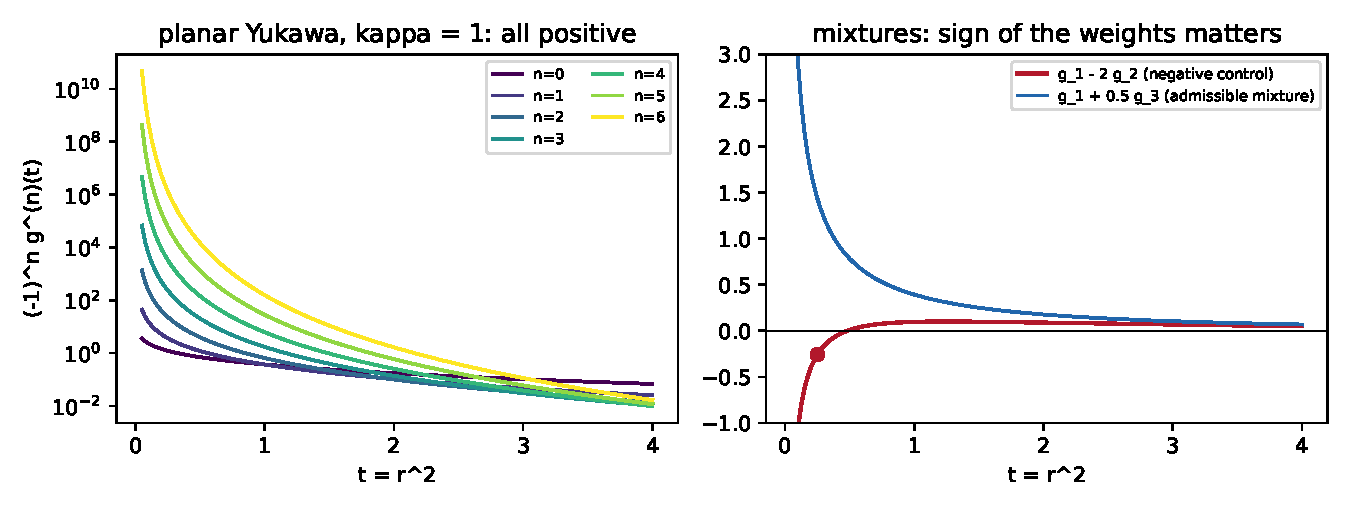
\includegraphics[width=\textwidth]{figures/fig_signs.pdf}
\caption{\tier{X} illustration, not evidence (\texttt{make\_figures.py}, mpmath at 40 digits). Left: $(-1)^n
g_1^{(n)}(t)$ for $n=0,\dots,6$ on $t\in[0.05,4]$, all positive (smallest sampled value $\SigMin$). Right: the
admissible mixture $g_1+\tfrac12g_3$ and the negative control $g_1-2g_2$, which is negative at $t=\tfrac14$
(dot).}\label{fig:signs}
\end{figure}

\section{The Lean formalization \tier{A}, conditional}\label{sec:lean}

\paragraph{Files.} \texttt{formal\_cert/Autoresearch/Yukawa.lean} (197 lines; prior round, docstrings updated) and
\texttt{YukawaMix.lean} (233 lines; this contribution), with planted controls only in the separate files
\texttt{YukawaControls.lean} and \texttt{YukawaMixControls.lean}. Toolchain: openai/math's pinned Lean~4.34.1 and
Mathlib \texttt{d13f23b7}, via \texttt{scripts/certified\_numerics/lean\_pinned.py}. The listings above are cut from the
files by \texttt{gen\_listings.py} and are byte-verbatim; sha256 values are in Section~\ref{sec:repro}.

\paragraph{Axiom audit.} \texttt{Autoresearch.Yukawa} compiles with rc \RcYk{} and \texttt{Autoresearch.YukawaMix}
with rc \RcMix{}. Verbatim \verb|#print axioms| output:
\begin{Verbatim}[fontsize=\scriptsize,frame=single,framesep=1.5mm]
'AutoresearchYukawa.mul_sign' -> [propext, Classical.choice, Quot.sound]
'AutoresearchYukawa.admissible_mul' -> [propext, Classical.choice, Quot.sound]
'AutoresearchYukawa.admissible_congr' -> [propext, Classical.choice, Quot.sound]
'AutoresearchYukawa.phi_admissible' -> [propext, Classical.choice, Quot.sound]
'AutoresearchYukawa.yukawa_admissible' -> [propext, Classical.choice, Quot.sound]
'AutoresearchYukawa.triangular_yukawa_optimal' -> [propext, Classical.choice, Quot.sound]
'AutoresearchYukawa.c_not_admissible' -> [propext, Classical.choice, Quot.sound]
'AutoresearchYukawa.latticeEnergy_yukawa_lt_top' -> [propext, Classical.choice, Quot.sound]
\end{Verbatim}

\begin{Verbatim}[fontsize=\scriptsize,frame=single,framesep=1.5mm]
'AutoresearchYukawaMix.admissible_add' -> [propext, Classical.choice, Quot.sound]
'AutoresearchYukawaMix.admissible_smul' -> [propext, Classical.choice, Quot.sound]
'AutoresearchYukawaMix.admissible_zero' -> [propext, Classical.choice, Quot.sound]
'AutoresearchYukawaMix.admissible_sum' -> [propext, Classical.choice, Quot.sound]
'AutoresearchYukawaMix.latticeEnergy_lt_top_of_le_riesz3' -> [propext, Classical.choice, Quot.sound]
'AutoresearchYukawaMix.g_rescale' -> [propext, Classical.choice, Quot.sound]
'AutoresearchYukawaMix.yukawa_any_density' -> [propext, Classical.choice, Quot.sound]
'AutoresearchYukawaMix.yukawa_optimal_any_density' -> [propext, Classical.choice, Quot.sound]
'AutoresearchYukawaMix.latticeEnergy_yukawa_rho_lt_top' -> [propext, Classical.choice, Quot.sound]
'AutoresearchYukawaMix.yukawaMix_admissible' -> [propext, Classical.choice, Quot.sound]
'AutoresearchYukawaMix.triangular_yukawaMix_optimal' -> [propext, Classical.choice, Quot.sound]
'AutoresearchYukawaMix.latticeEnergy_yukawaMix_lt_top' -> [propext, Classical.choice, Quot.sound]
'AutoresearchYukawaMix.yukawaMix_optimal_any_density' -> [propext, Classical.choice, Quot.sound]
'AutoresearchYukawaMix.latticeEnergy_yukawaMix_rho_lt_top' -> [propext, Classical.choice, Quot.sound]
'AutoresearchYukawaMix.two_length_admissible' -> [propext, Classical.choice, Quot.sound]
'AutoresearchYukawaMix.signedMix_not_admissible' -> [propext, Classical.choice, Quot.sound]
\end{Verbatim}


\paragraph{Controls.} The planted \texttt{sorry} and the planted axiom are caught in both control files (rc
\RcYkCtl{} and \RcMixCtl{}). The positive instances evaluate the theorems at concrete parameters, so the hypotheses are
satisfiable:
\begin{Verbatim}[fontsize=\scriptsize,frame=single,framesep=1.5mm]
.../YukawaControls.lean:7:8: warning: declaration uses `sorry`
'AutoresearchYukawaControls.ctl_sorry' -> [sorryAx]
'AutoresearchYukawaControls.ctl_axiom' -> [AutoresearchYukawaControls.ctl_cheat]
\end{Verbatim}

\begin{Verbatim}[fontsize=\scriptsize,frame=single,framesep=1.5mm]
.../YukawaMixControls.lean:11:8: warning: declaration uses `sorry`
'AutoresearchYukawaMixControls.ctl_sorry' -> [sorryAx]
'AutoresearchYukawaMixControls.ctl_axiom' -> [AutoresearchYukawaMixControls.ctl_cheat]
'AutoresearchYukawaMixControls.pos_two_length' -> [propext, Classical.choice, Quot.sound]
'AutoresearchYukawaMixControls.pos_mix_rho3_finite' -> [propext, Classical.choice, Quot.sound]
'AutoresearchYukawaMixControls.pos_yukawa_rho2' -> [propext, Classical.choice, Quot.sound]
\end{Verbatim}

A forbidden-token grep (\texttt{sorry}, \texttt{admit}, \texttt{axiom}, \texttt{native\_decide},
\texttt{implemented\_by}, \texttt{extern}, \texttt{unsafe}) of the two claimed files finds nothing.

\paragraph{Independent recompiles (producer $\ne$ verifier).} For \texttt{Yukawa.lean} a separate agent instance
recompiled a verbatim copy and audited the statements adversarially (verdict ACCEPT, \texttt{H2/verification.md}). It
proved $g_\kappa(r^2)=e^{-\kappa r}/r$ and showed that the definitions are upstream's (\texttt{Iff.rfl}/\texttt{rfl}).
That audit was of the prior-round bytes (sha256 \texttt{43e2df3f\dots}). The current file (\texttt{a16397de\dots})
differs only in docstrings, by \texttt{diff}, and its rebuilt axiom output is identical. For
\texttt{YukawaMix.lean}, the agent writing this paper (not its producer) compiled a verbatim copy with a verifier block
appended (rc \RcVer{}). The block contains: \texttt{rfl} unfoldings of \lean{yukawaMix}, $g$ and \lean{DensityRho}; the
pointwise identity $g_\kappa(r^2)=e^{-\kappa r}/r$; statement pins; a three-length non-vacuity instance with weights
$(1,2,\tfrac12)$ and screenings $(\tfrac12,1,3)$; positivity of that mixture; and a planted \texttt{sorry} of its own:
\begin{Verbatim}[fontsize=\scriptsize,frame=single,framesep=1.5mm]
.../VerifyYukawaMix.lean:278:8: warning: declaration uses `sorry`
'VerifierH2Mix.v_three_length_finite' -> [propext, Classical.choice, Quot.sound]
'VerifierH2Mix.v_mix_pos' -> [propext, Classical.choice, Quot.sound]
'VerifierH2Mix.v_planted' -> [propext, sorryAx, Classical.choice, Quot.sound]
'VerifierH2Mix.v_planted_use' -> [propext, sorryAx, Classical.choice, Quot.sound]
\end{Verbatim}

A third, independent AI audit of the whole preprint recompiled byte copies of both claimed files and both control files
(all rc~0, every claimed theorem within the allowlist) and caught a planted \texttt{sorry} and a planted axiom in a
file of its own. All audits were carried out by AI agents. No human has audited statement adequacy, so every Tier~A row of the ledger
carries the flag \texttt{LEDGER\_UNAUDITED\_TIER\_A}.

\section{Physics: what the theorem says and does not say}\label{sec:physics}

\paragraph{System \tier{C}.} Point particles confined to a plane, interacting pairwise by $V(r)=Q^2e^{-r/\lambda_D}/r$:
the screened Coulomb (Yukawa) interaction of charged grains in a dusty-plasma monolayer or of charged
colloids at an interface or in a thin cell. The screening is three-dimensional, from the surrounding plasma
or electrolyte; this is the standard 2D Yukawa model, not the 2D Debye--H\"uckel kernel $K_0$.

\paragraph{Units and regime \tier{C}.} Lengths are in units of $\ell=\rho^{-1/2}$, so at density one $\ell=1$ and
the nearest-neighbour spacing is $a=\sqrt{2/\sqrt3}\approx1.075$. Energies are in units of $Q^2/\ell$, and
$\kappa=\ell/\lambda_D$. After the rescaling of Step~8, the single dimensionless parameter is $\kappa\ell$. With a
Wigner--Seitz radius defined by $\pi a_{\rm WS}^2\rho=1$, $\kappa a_{\rm WS}=\kappa\ell/\sqrt\pi$ (our arithmetic). The model is classical, at
temperature zero, with no substrate, no confinement, no 3D motion and no many-body (non-pairwise) screening
corrections.

\paragraph{What is proved \tier{A}, conditional.} For every $\kappa>0$, every density $\rho>0$ and every finite
nonnegative mixture of screening lengths, no locally finite planar configuration of that density has lower
($\liminf$ disk-averaged) energy than the triangular lattice, and the lattice's energy is finite. A mixture
$\sum_iw_ie^{-\kappa_ir}/r$ describes, for example, a two-population screening cloud. Unlike the single-$\kappa$ case,
a mixture is not reduced to one parameter by rescaling, since the ratios $\kappa_i/\kappa_j$ are preserved.

\paragraph{What is not said.} (1) Uniqueness: upstream identifies the minimum value, not all minimisers \tier{L}~\cite{oai};
the lattice with a vacancy has the same energy, since ``removing a single particle changes neither the density nor
the energy'' \tier{L}~\cite[arXiv version, p.~8, remark after Thm.~1.4]{ckmrv}. (2) Finite temperature, melting, dynamics or the path by which a
system reaches the lattice. (3) $K_0$ or any potential outside the admissible class, including truncated or
shifted-force versions of $V$, which are not completely monotone. (4) Mixtures with a negative weight (Step~9b): the theorem does not apply to them, and whether the lattice minimises
their energy is left open.
(5) Novelty of the mathematics: complete monotonicity of $e^{-\kappa r}/r$ in $r^2$ and the cone and product closure
of completely monotone functions are classical. What is new is the kernel-checked corollary inside upstream's
framework.

\paragraph{The factor-2 convention \tier{C}.} Upstream's \lean{latticeEnergy} is $\sum_{a\ne0}g(|a|^2)$ over ordered
pairs. The numerics report the energy per particle $\tfrac12\sum_{a\ne0}V(|a|)$. So the Lean lattice energy at
$\kappa=1$ corresponds to $2\times\ETriOne=\TwiceTriOne$, and at $\kappa=2$ to $\TwiceTriTwo$. The ordering, which is
all the theorem concerns, is the same in both conventions.

\section{Numerics with rusty-SUNDIALS \tier{X}}\label{sec:numerics}

\paragraph{Why.} An earlier CVODE study of the Yukawa crystal~\cite{uo2} used a shifted-force cut at $r_c=8$. The
textbook's editor's note~\cite{txt} recorded the resulting erratum: the cut lowers the energy per particle by about
$1.8\times10^{-2}$ at $\kappa=1$, more than the square--triangular gap, and the cut potential is not completely
monotone. We redo the computation with the exact potential.

\paragraph{Method.} Crate \texttt{qf-yukawa-crystal} of rusty-SUNDIALS~\cite{rusty}, new module \texttt{src/exact.rs}.
(a) Lattice sums $\tfrac12\sum_{0<|v|<R}V(|v|)$, sorted and compensated, with a rigorous Voronoi-cell tail bound: for
decreasing $V$ the tail beyond $R$ is at most $(\pi/A)(1+\delta/(R-2\delta))e^{-\kappa(R-2\delta)}/\kappa$ per particle
($\delta$ the cell circumradius, $A$ the cell area). With $R=\ROne$ ($\kappa=1$) and $R=\RTwo$ ($\kappa=2$) the bound is at
most $\TailOne$ and $\TailTwo$. (b) An independent Ewald-type splitting of the same sum, from
$e^{-\kappa r}/r=\tfrac{2}{\sqrt\pi}\int_0^\infty e^{-r^2s^2-\kappa^2/(4s^2)}\,ds$, with closed-form \texttt{erfc} terms.
(c) A periodic box in which each pair interacts with all its periodic images within $R$, including each particle's
own images, with analytic energy, force and Hessian. Relaxation uses this repository's CVODE (BDF, analytic Jacobian
$=-$Hessian, rtol $10^{-10}$, atol $10^{-12}$, force tolerance $10^{-9}$), and minima are checked by the Hessian spectrum.
Initial conditions and protocol are the published ones~\cite{uo2}; annealing was not re-run with the exact potential.

\paragraph{Results: lattice energies.} Energy per particle at density one (Table~\ref{tab:lat}). The exact values
differ from the published shifted-force ones by the erratum amounts. The square--triangular gap changes only by
$\GapChOne$ ($\kappa=1$) and $\GapChTwo$ ($\kappa=2$); the triangular lattice stays lower.

\begin{table}[!ht]\centering\footnotesize\setlength{\tabcolsep}{4pt}
\begin{tabular}{llllll}
\toprule
$\kappa$ & lattice & shifted force, $r_c=8$ (publ.) & exact (this work) & exact $-$ publ. & gap sq$-$tri, exact\\
\midrule
1 & triangular & \SfTriOne & \ETriOne & $\DTriOne$ & $\GapExOne$\\
1 & square & \SfSqOne & \ESqOne & $\DSqOne$ & \\
2 & triangular & \SfTriTwo & \ETriTwo & $\DTriTwo$ & $\GapExTwo$\\
2 & square & \SfSqTwo & \ESqTwo & $\DSqTwo$ & \\
\bottomrule
\end{tabular}
\caption{\tier{X} Lattice energies per particle ($\tfrac12\sum$ convention). Published gaps: $\GapSfOne$ ($\kappa=1$),
$\GapSfTwo$ ($\kappa=2$). Source: \texttt{data/exact\_refs.jsonl}.}\label{tab:lat}
\end{table}

\paragraph{Positive controls.} (P1) An independent mpmath computation at \MpDps{} digits, sharing no code with the
Rust, by direct summation with tail below $2\times10^{-28}$ and by an Ewald splitting. Direct and Ewald agree to
$\MpMaxEwald$, and the Rust double-precision values agree with mpmath to at most $\MpMaxRust$ (threshold $10^{-9}$).
(P2) The image-summed periodic box holding the perfect lattice equals the infinite-lattice sum to $\BoxDiffOne$
($\kappa=1$) and $\BoxDiffTwo$ ($\kappa=2$). The self-image term, $\SelfImgOne$ at $\kappa=1$, is included. (P3) Unit
tests check direct sum against Ewald splitting, and force and Hessian against finite differences.

\paragraph{Negative controls.} (N1) The published shifted-force lattice energies fail the $10^{-9}$ agreement test
against the exact values, by exactly the erratum amounts. (N2) The perfect square lattice in a $17\times17$ box under
the exact potential has \SadNegOne{} ($\kappa=1$) and \SadNegTwo{} ($\kappa=2$) negative Hessian modes, the same counts
as published. After a perturbation it relaxes to $\SadAfterOne$ and $\SadAfterTwo$ above $e_{\rm tri}$. (N3) Runs in
the incommensurate $17\times17$ box, which cannot hold the triangular lattice, stay above it.

\paragraph{Results: relaxed configurations.} We took \NRelax{} relaxed stages from 21 published runs: \NRelaxOne{} of
the 50 published stages at $\kappa=1$ and \NRelaxTwo{} of the 100 at $\kappa=2$. Each stage was first re-run with the
published shifted-force protocol, and \NSfRepro{} of \NRelax{} reproduce their published energies to below
$10^{-13}$. Each was then re-relaxed under the exact potential, and \NConv{} of \NRelax{} converge. \NBelow{} fall below the
exact triangular energy beyond f64 resolution, and \NNegModes{} have negative Hessian modes. The test is
$e-e_{\rm tri}<0$ with zero tolerance. \NZeroGap{} stage (\ZeroGapStage) relaxes to the perfect lattice and sits at
gap exactly $0$; at that point the outcome is set by rounding, not by the physics, since the perfect lattice in the
$\kappa=1$ box differs from the lattice sum by $\TriBoxDiffOne$. The gaps to $e_{\rm tri}$ change by at most
$\MaxGapChOne$ at $\kappa=1$, about 860 times less than the smallest nonzero gap ($\MinGapOne$), and by at most
$\MaxGapChTwo$ at $\kappa=2$. The gap changes are computed from 7-digit printed gaps. Defect counts are unchanged
(Table~\ref{tab:relax}, Figure~\ref{fig:relax}). This is consistent with the theorem for these seeds and is not
evidence for it.

\begin{table}[!ht]\centering\scriptsize\setlength{\tabcolsep}{3pt}
\begin{tabular}{llllllll}
\toprule
$\kappa$ & run & stage & gap, shifted force & gap, exact & change & defects sf/exact & neg.\ modes\\
\midrule
1 & \texttt{incommensurate\_00} & anneal quench & $4.9630\times10^{-4}$ & $4.9660\times10^{-4}$ & $2.9\times10^{-7}$ & 4/4 & 0 \\
1 & \texttt{incommensurate\_00} & quench & $7.5353\times10^{-4}$ & $7.5365\times10^{-4}$ & $1.3\times10^{-7}$ & 4/4 & 0 \\
1 & \texttt{incommensurate\_01} & quench & $7.9177\times10^{-4}$ & $7.9218\times10^{-4}$ & $4.0\times10^{-7}$ & 4/4 & 0 \\
1 & \texttt{oc20\_00} & anneal quench & $4.7942\times10^{-4}$ & $4.7995\times10^{-4}$ & $5.3\times10^{-7}$ & 0/0 & 0 \\
1 & \texttt{oc20\_00} & quench & $4.5835\times10^{-4}$ & $4.5856\times10^{-4}$ & $2.1\times10^{-7}$ & 0/0 & 0 \\
1 & \texttt{oc20\_01} & quench & $6.6930\times10^{-4}$ & $6.6960\times10^{-4}$ & $3.0\times10^{-7}$ & 4/4 & 0 \\
1 & \texttt{oc20\_02} & quench & $8.4414\times10^{-4}$ & $8.4430\times10^{-4}$ & $1.6\times10^{-7}$ & 4/4 & 0 \\
1 & \texttt{uniform\_00} & anneal quench & $3.1086\times10^{-14}$ & $0$ & $-3.1\times10^{-14}$ & 0/0 & 0 \\
1 & \texttt{uniform\_00} & quench & $9.5804\times10^{-4}$ & $9.5828\times10^{-4}$ & $2.4\times10^{-7}$ & 4/4 & 0 \\
1 & \texttt{uniform\_01} & quench & $1.2743\times10^{-3}$ & $1.2742\times10^{-3}$ & $-1.8\times10^{-7}$ & 8/8 & 0 \\
1 & \texttt{uniform\_02} & quench & $6.6930\times10^{-4}$ & $6.6960\times10^{-4}$ & $3.0\times10^{-7}$ & 4/4 & 0 \\
2 & \texttt{incommensurate\_00} & quench & $3.7772\times10^{-4}$ & $3.7772\times10^{-4}$ & $3.0\times10^{-10}$ & 4/4 & 0 \\
2 & \texttt{incommensurate\_01} & quench & $3.7881\times10^{-4}$ & $3.7881\times10^{-4}$ & $3.0\times10^{-10}$ & 4/4 & 0 \\
2 & \texttt{incommensurate\_02} & quench & $9.1304\times10^{-4}$ & $9.1304\times10^{-4}$ & $0$ & 8/8 & 0 \\
2 & \texttt{oc20\_00} & quench & $1.7420\times10^{-3}$ & $1.7420\times10^{-3}$ & $0$ & 24/24 & 0 \\
2 & \texttt{oc20\_01} & quench & $1.8583\times10^{-3}$ & $1.8583\times10^{-3}$ & $0$ & 24/24 & 0 \\
2 & \texttt{oc20\_02} & quench & $5.0488\times10^{-4}$ & $5.0488\times10^{-4}$ & $2.0\times10^{-10}$ & 4/4 & 0 \\
2 & \texttt{oc20\_03} & quench & $6.5753\times10^{-4}$ & $6.5753\times10^{-4}$ & $-1.0\times10^{-10}$ & 4/4 & 0 \\
2 & \texttt{oc20\_04} & quench & $1.3550\times10^{-3}$ & $1.3550\times10^{-3}$ & $0$ & 12/12 & 0 \\
2 & \texttt{uniform\_00} & quench & $6.6789\times10^{-4}$ & $6.6789\times10^{-4}$ & $1.0\times10^{-10}$ & 4/4 & 0 \\
2 & \texttt{uniform\_01} & quench & $6.0271\times10^{-4}$ & $6.0271\times10^{-4}$ & $-3.0\times10^{-10}$ & 4/4 & 0 \\
2 & \texttt{uniform\_02} & quench & $7.2333\times10^{-5}$ & $7.2333\times10^{-5}$ & $1.2\times10^{-10}$ & 0/0 & 0 \\
2 & \texttt{uniform\_03} & quench & $2.3767\times10^{-3}$ & $2.3767\times10^{-3}$ & $0$ & 34/34 & 0 \\
2 & \texttt{uniform\_04} & quench & $7.2333\times10^{-5}$ & $7.2333\times10^{-5}$ & $1.2\times10^{-10}$ & 0/0 & 0 \\
\bottomrule

\end{tabular}
\caption{\tier{X} Relaxed stages: gap $e-e_{\rm tri}$, each potential against its own $e_{\rm tri}$. Generated from
\texttt{data/exact\_summary.json} by \texttt{gen\_numbers.py}.}\label{tab:relax}
\end{table}

\begin{figure}[!ht]\centering
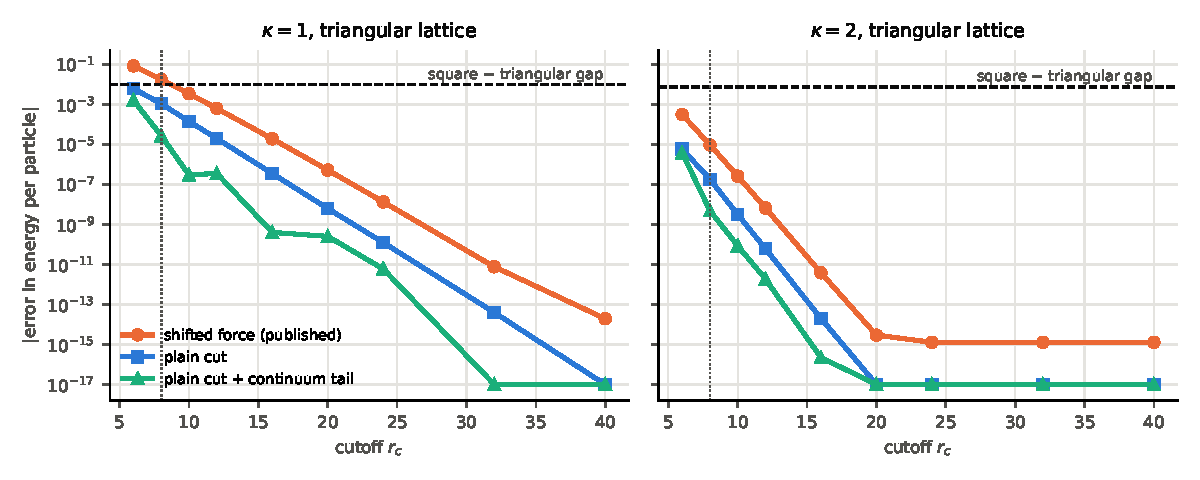
\includegraphics[width=0.49\textwidth]{data/fig_cutoff_sweep.pdf}\hfill
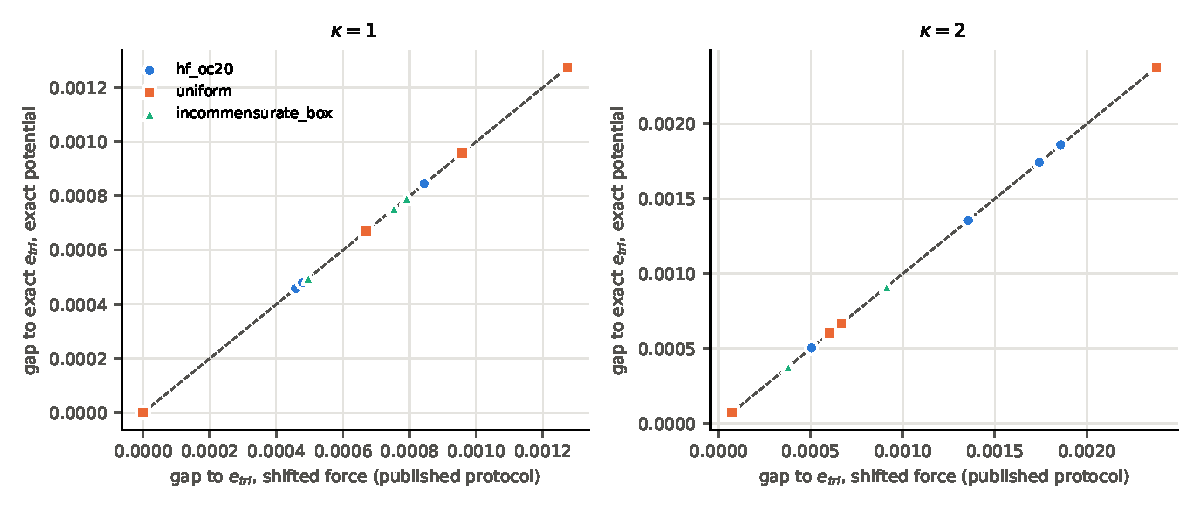
\includegraphics[width=0.49\textwidth]{data/fig_relaxed_gaps.pdf}
\caption{\tier{X} Left: error of shifted-force, plain-cut and plain-plus-continuum-tail triangular-lattice energies
against the converged value, versus $r_c$, with the square--triangular gap for reference (points at $10^{-17}$ are exact
zeros clipped for the log axis). Right: published shifted-force gap versus exact gap per relaxed stage. Both are
generated by \texttt{scripts/exact\_figures.py} in the rusty-SUNDIALS crate.}\label{fig:relax}
\end{figure}

\section{Hugging Face dataset illustration}\label{sec:hf}

\paragraph{What we looked for \tier{C}.} On 2026-10-25 we searched the Hub (public, unauthenticated) for ``dusty
plasma'', ``dusty-plasma'', ``complex plasma'', ``colloid'', ``colloidal'', ``yukawa'' and ``wigner crystal''. No
dataset of dusty-plasma or colloid particle positions was found. That is absence by search, not proof. The two hits were
\texttt{YangyangTan/yukawa-2d-diffusion} (lattice-field-theory configurations of a Yukawa \emph{coupling}, a name
collision) and \texttt{VIJAYALAKSHMI10/Colloidal\_model} (no license, empty card). Only their metadata was downloaded.

\paragraph{What we used \tier{X}.} The disordered initial conditions of the published study come from
\texttt{colabfit/OC20\_IS2RES\_val\_id}~\cite{oc20}, license \OcLicense{}, shard \texttt{co/co\_10.parquet}
(\OcBytes{} bytes). The prior round had not recorded a revision. The local file's sha256 \texttt{\OcSha} equals the Hub
LFS sha256 at revision \texttt{\OcRev}, so the initial conditions are traceable to that revision by content. The
original download date was not recorded; the local file's modification time, \OcMtime{} UTC, is a latest possible
date. Random OC20 structures were rotated in 3D, projected onto the plane, rescaled, and
accepted with a minimum separation. In Table~\ref{tab:relax}, runs \texttt{oc20\_*} start from them.

\paragraph{What it shows, and caveats.} The dataset supplies realistic-looking \emph{disorder}, not physics: catalyst
adsorbate geometries have nothing to do with screened Coulomb particles. Starting from them, every exact-potential
relaxation stays above the triangular energy, as the theorem requires. It illustrates the statement and tests no
part of it. A real dusty-plasma or colloid trajectory dataset would allow a more meaningful illustration; none is
on the Hub.

\section{Limitations}\label{sec:limits}

(1) Every optimality statement is conditional on upstream \lean{universal_energy_minimum} (AI-generated,
Comparator-accepted, not peer reviewed) and on the fidelity of its definitions to the physical question
(\lean{energy} as a $\liminf$ of disk averages, \lean{DensityOne} via centred disks). (2) Statement adequacy was audited
by AI agents only; \LedgerFlags{} Tier~A rows are flagged. (3) The mathematics is classical; the contribution is
formal. (4) The every-density result for a single $\kappa$ is a reparametrisation; the energy-level scaling is not stated
in Lean. (5) Not covered: $K_0$, infinite (integral) mixtures, negative weights, uniqueness, finite temperature.
(6) Numerics: a subset of the published stages (\NRelaxOne/50 at $\kappa=1$, \NRelaxTwo/100 at $\kappa=2$, quench only
at $\kappa=2$); annealing not re-run with the exact potential, so the published $\kappa=1$ dynamics failure is untested;
for the periodic box only a continuum tail estimate is reported (the rigorous bound covers the lattice sums). (7)
Numbers are floating point and support no claim. (8) The rusty-SUNDIALS commits are local and not pushed; the
AutoevolveAI Lean files are uncommitted at the time of writing; they must be committed before any archival upload so
that the sha256 values of Section~\ref{sec:repro} can be reproduced from git. (9) \texttt{elenchus\_check.py}
(source-level vacuity scan) gives no usable result on these files: the independent auditor ran it and it returned only
\texttt{COMPILE\_ERROR}, because its Lean~4.34.0-rc2 toolchain cannot see the pinned 4.34.1 stack. The kernel
footprint checks, recompiles and planted controls with the pinned toolchain replace it.

\section{Reproducibility}\label{sec:repro}

\begin{Verbatim}[fontsize=\scriptsize,frame=single,framesep=1.5mm]
# Lean (AutoevolveAI worktree openai-math-discovery, HEAD db794dd98d12c2a79702eab5651ae7c36a35ea27; files uncommitted)
taskset -c 4-7 python3 scripts/certified_numerics/lean_pinned.py compile formal_cert/Autoresearch/Yukawa.lean \
    --olean Autoresearch.Yukawa --json-out results/autoresearch/2026-10-25/H2/contribution/compile_yukawa.json
taskset -c 4-7 python3 scripts/certified_numerics/lean_pinned.py compile formal_cert/Autoresearch/YukawaMix.lean \
    --olean Autoresearch.YukawaMix --json-out results/autoresearch/2026-10-25/H2/contribution/compile_yukawamix.json
#   then YukawaControls.lean, YukawaMixControls.lean, and contribution/verify/VerifyYukawaMix.lean (no --olean)
# sha256: Yukawa.lean            a16397de179837dd2119cf09c1b3086db7650b9b8bbaeb322f2d531936c033cf
#         YukawaMix.lean         6a940a7cb1b4b25391a8fb6348873e04e4219501877c3a037760cd6f31b374c6
#         YukawaControls.lean    ff7f11da15e3cfbe9dcd612397db2effbfdd99a89da876607ded9aa0d25740ff
#         YukawaMixControls.lean 028a39361e23fe20ae510ed84300ad223087f3dff3df0e7edb749a30c93cbbf3
#         VerifyYukawaMix.lean   f347d67df563268ff6cc0062d9fdd95ae76650275424648a2f319b96e235ea0e
# Numerics: rusty-SUNDIALS branch physics/ar-yukawa-2026-10-25, base 47ef5044c10b04c64d8c86f483f1aa47c400ab28,
#   code cc5a8aed81b3228bd9e9eb69f2c326f926903a34, results 7f2a45c32a9eb9722ca36c334329cb7a5a541951 (not pushed)
CARGO_TARGET_DIR=<target> cargo build --release -j 2 --offline -p qf-yukawa-crystal
yukawa_crystal exact-refs <crate>        # lattice energies, sweep, box controls
yukawa_crystal exact-relax <kappa> <nrun> <anneal> <first>     # see scripts/run_exact_relax.sh
yukawa_crystal exact-saddle <crate>      # square-lattice negative control
python -I scripts/mpmath_lattice_control.py <crate> <out.json>  # 40-digit positive control
bash scripts/check_crate.sh              # fmt, clippy, tests: 24 passed, 0 failed, 1 ignored
#   (re-run at revision, output in H2/contribution/check_crate_stage5.txt, same counts)
# Paper (papers/ar_yukawa_crystal): python -I gen_listings.py; python -I make_figures.py;
#   python -I ledger/build_ledger.py; python -I gen_numbers.py (re-runs the Elenchus gate); pdflatex main.tex (twice)
python3 <Elenchus>/tools/ledger.py ledger/ledger.json --evidence-dir ledger/evidence --json   # Elenchus c9ae8cd
\end{Verbatim}

\paragraph{Disclosure.} This work was produced by AI agents (Claude, Anthropic) under the author's direction: the Lean
proofs, the Rust code, the numerics, the audits and this text. The author is responsible for the content. No human
expert has reviewed it; red-team review is invited.

\begin{thebibliography}{9}
\bibitem{oai} OpenAI, Universal optimality of the triangular lattice, OpenAI Math Release preprint, 2026-09-23,
\url{https://github.com/openai/math} (commit \texttt{fd4aeeb2}).
\bibitem{ckmrv} H.~Cohn, A.~Kumar, S.~D.~Miller, D.~Radchenko, M.~Viazovska, Universal optimality of the $E_8$ and
Leech lattices and interpolation formulas, Ann.\ of Math.\ 196 (2022) 983--1082, doi:10.4007/annals.2022.196.3.3;
arXiv:1902.05438 (page numbers cited here are those of the arXiv version).
\bibitem{d12} X.~Callens, Riesz-energy, finiteness and every-density corollaries of the openai/math planar
universal-optimality theorem, kernel-checked in Lean 4, Zenodo (2026), doi:10.5281/zenodo.23285631.
\bibitem{uo2} X.~Callens, Planar universal optimality, tiered: kernel-checked consequences, a non-uniqueness theorem,
and a CVODE $N$-body consistency check for the Yukawa interaction, preprint v2, Zenodo (2026), doi:10.5281/zenodo.23293429.
\bibitem{txt} X.~Callens, The Triangular Lattice and Universal Optimality (textbook, with editor's note), Zenodo
(2026), doi:10.5281/zenodo.23295142.
\bibitem{elenchus} X.~Callens, SocrateAI-Scientific-Elenchus,
\url{https://github.com/xaviercallens/SocrateAI-Scientific-Elenchus} (commit \texttt{c9ae8cd}).
\bibitem{rusty} X.~Callens, rusty-SUNDIALS, \url{https://github.com/xaviercallens/rusty-SUNDIALS}.
\bibitem{oc20} Hugging Face dataset \texttt{colabfit/OC20\_IS2RES\_val\_id} (CC-BY-4.0), revision
\texttt{\OcRev}, dataset doi:10.60732/b4005525; L.~Chanussot et al., The Open Catalyst 2020 (OC20) dataset and
community challenges, arXiv:2010.09990; journal version doi:10.1021/acscatal.0c04525 (as given on the dataset card).
\end{thebibliography}
\end{document}
